% ПРОЧИТАЙ МЕНЯ
% ПРОЧИТАЙ МЕНЯ
% ПРОЧИТАЙ МЕНЯ
%
% В этом файле вы описываете задачи из контеста
% Условия можно вставить в виде фотографий
% В идеях нужно написать хотя бы два-три предложения о задаче
% Если задача довольно трудная, описание идеи должно быть подробным
% Комментарии в исходном коде приветствуются
% Положение тоже можно фотографией
%
% ПРОЧИТАЙ МЕНЯ
% ПРОЧИТАЙ МЕНЯ
% ПРОЧИТАЙ МЕНЯ

\section{Отчёт обучающегося по практике}

\subsection*{Codeforces Round \#768 (Div. 2)}
\begin{center}
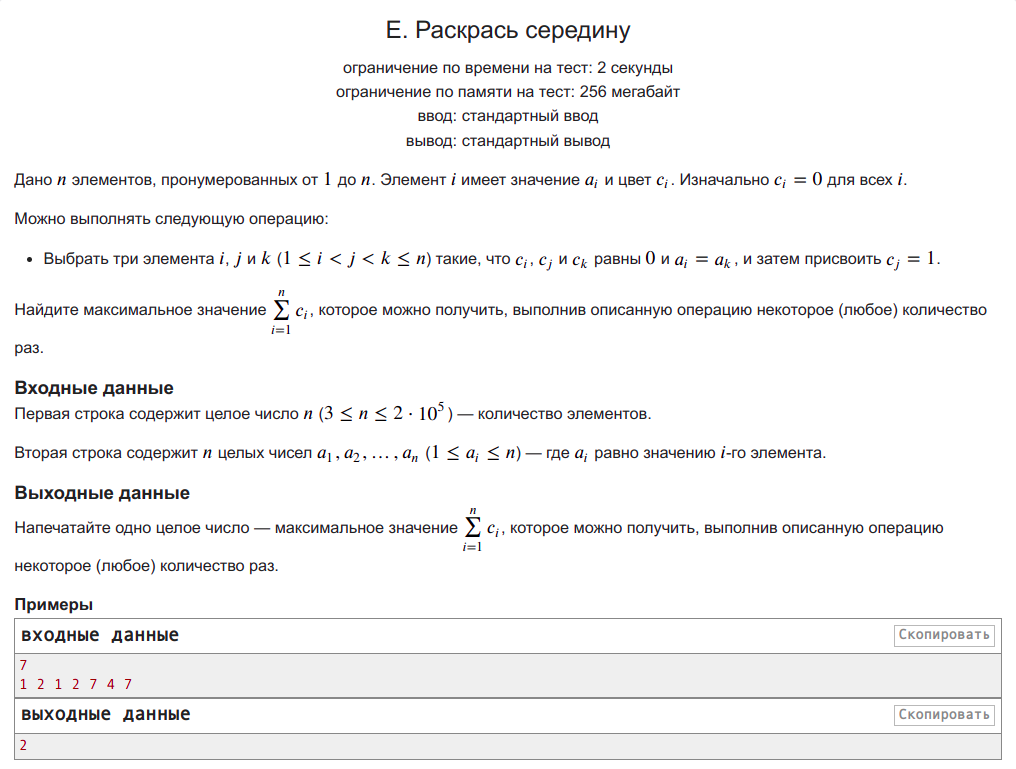
\includegraphics[width=\textwidth]{statements/sample-cf.png}
\end{center}
\subsubsection*{Идея решения}
Описать идею решения, оценить сложность, сравнить с другими возможными идеями.

{\bfseries \large Например}

Переборное решение работает $O(n!)$, это очень долго. Использую метод динамического программирования, $dp_i$ --- это минимальное количество белочек при условии чего-то там для $i$ веточек. Это позволяет решить задачу за $O(n ^ 2)$. Дерево отрезков с отложенными обновлениями позволяет улучшить асимптотику до $O(n \cdot \log{n})$, так как все операции с деревом соврешаются за $O(\log{n})$.

\subsubsection*{Исходный код}
\textit{Исходный код необходимо комментировать, но не более 25\% строк}
\lstinputlisting{src/sample-cf-e.cpp}

\subsubsection*{Фрагмент турнирной таблицы контеста}
\begin{center}
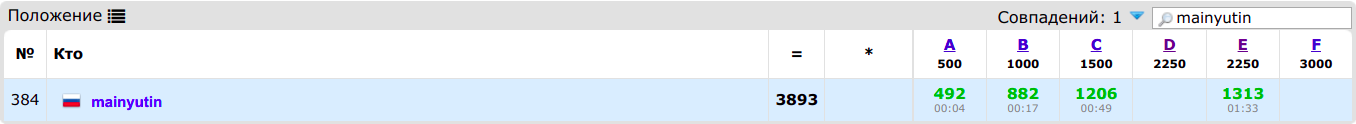
\includegraphics[width=\textwidth]{standings/sample-cf.png}\newline\noindent
\end{center}

\subsubsection*{Выводы}
Задача решена. \textbf{ИЛИ} Задача дорешана. \textbf{ИЛИ} Не принята чекером.

Ошибки, неудачи, как они преодолевались.

{\bfseries \large Например}

Задача решена. Основные события процесса отладки: неправильный ответ на претесте 3, исправил дерево отрезков.

\vspace{16pt}
\textit{Если задач много (более одной на контест), то часть отчёта может быть представлена в электронном виде (на компакт диске или на плоской флешке, оглавление прилагаемого носителя должно быть распечатано рекурсивным обходом и должно однозначно интерпретироваться как контесты и задачи). На носитель следует поместить журнал в формате pdf и в виде исходного кода (в случае LaTeX должен быть makefile). Для каждого контеста следует завести отдельную директорию (например: в папку \enquote{20220630} поместить файлы \enquote{a.cpp}, \enquote{b.cpp} и условия задач).}

\pagebreak
